% answers.tex —— 2012 年·全国新课标卷·文科 · 参考答案与详细解析片段
% 由 tools/generate_projects.py 依来源总账自 2012/2012_数学真题_全国新课标文_试题.md + 2012/2012_数学真题_全国新课标文_解析正文.md + 2012/2012_数学真题_全国新课标文_答案要点.md 生成，勿手改（改源 MD 后重跑）


\begin{answer}
\gksolhead{1}{}

\textbf{题目}：

已知集合 $A=\{x\mid x^2-x-2<0\}$，$B=\{x\mid -1<x<1\}$，则\mbox{（　　）}

\begin{gkopts}(2)
\task （A）$A\subsetneqq B$
\task （B）$B\subsetneqq A$
\task （C）$A=B$
\task （D）$A\cap B=\varnothing$
\end{gkopts}

\Needspace{4\baselineskip}
\textbf{解析}

$x^2-x-2<0$ 的解集为 $(-1,2)$，而 $B=(-1,1)$，所以 $B\subsetneqq A$，选 B。

\gkanswer{答案：B}

\end{answer}
\begin{answer}
\gksolhead{2}{}

\textbf{题目}：

复数 $z=\dfrac{-3+i}{2+i}$ 的共轭复数是\mbox{（　　）}

\begin{gkopts}(4)
\task （A）$2+i$
\task （B）$2-i$
\task （C）$-1+i$
\task （D）$-1-i$
\end{gkopts}

\Needspace{4\baselineskip}
\textbf{解析}

\nopagebreak[4]
\[
z=\frac{(-3+i)(2-i)}{(2+i)(2-i)}=-1+i,
\]
故 $\overline z=-1-i$，选 D。

\gkanswer{答案：D}

\end{answer}
\begin{answer}
\gksolhead{3}{}

\textbf{题目}：

在一组样本数据 $(x_1,y_1),(x_2,y_2),\cdots,(x_n,y_n)$（$n\geqslant2$，$x_1,x_2,\cdots,x_n$ 不全相等）的散点图中，若所有样本点 $(x_i,y_i)$（$i=1,2,\cdots,n$）都在直线 $y=\dfrac12x+1$ 上，则这组样本数据的样本相关系数为\mbox{（　　）}

\begin{gkopts}(4)
\task （A）$-1$
\task （B）$0$
\task （C）$\dfrac12$
\task （D）$1$
\end{gkopts}

\Needspace{4\baselineskip}
\textbf{解析}

所有样本点满足 $y_i=\frac12x_i+1$，且 $x_i$ 不全相等，样本点完全落在斜率为正的直线上，样本相关系数为 $1$，选 D。

\gkanswer{答案：D}

\end{answer}
\begin{answer}
\gksolhead{4}{}

\textbf{题目}：

设 $F_1,F_2$ 是椭圆 $E:\dfrac{x^2}{a^2}+\dfrac{y^2}{b^2}=1$（$a>b>0$）的左、右焦点，$P$ 为直线 $x=\dfrac{3a}{2}$ 上一点，$\triangle F_2PF_1$ 是底角为 $30^\circ$ 的等腰三角形，则 $E$ 的离心率为\mbox{（　　）}

\begin{gkopts}(4)
\task （A）$\dfrac12$
\task （B）$\dfrac23$
\task （C）$\dfrac34$
\task （D）$\dfrac45$
\end{gkopts}

\Needspace{4\baselineskip}
\textbf{解析}

\Needspace{5\baselineskip}
令焦半距为 $c$，取 $P$ 在 $x$ 轴上方。等腰三角形的底角在 $F_1,F_2$ 处为 $30^\circ$，故
\nopagebreak[4]
\[
\tan30^\circ=\frac{y_P}{\frac32a+c},\qquad
PF_2=F_1F_2=2c.
\]
\Needspace{5\baselineskip}
代入 $y_P=(\frac32a+c)/\sqrt3$，得到
\nopagebreak[4]
\[
\left(\frac32a-c\right)^2+\frac{(\frac32a+c)^2}{3}=4c^2,
\]
即 $\frac32a=2c$。所以离心率 $e=c/a=3/4$，选 C。

\gkanswer{答案：C}

\end{answer}
\begin{answer}
\gksolhead{5}{}

\textbf{题目}：

已知正三角形 $ABC$ 的顶点 $A(1,1)$，$B(1,3)$，顶点 $C$ 在第一象限，若点 $(x,y)$ 在 $\triangle ABC$ 内部，则 $z=-x+y$ 的取值范围是\mbox{（　　）}

\begin{gkopts}(4)
\task （A）$(1-\sqrt3,2)$
\task （B）$(0,2)$
\task （C）$(\sqrt3-1,2)$
\task （D）$(0,1+\sqrt3)$
\end{gkopts}

\Needspace{4\baselineskip}
\textbf{解析}

\Needspace{5\baselineskip}
由 $AB=2$ 且 $C$ 在第一象限，$C=(1+\sqrt3,2)$。线性函数 $z=-x+y$ 在三角形内部的值严格介于三个顶点处的值之间，而
\nopagebreak[4]
\[
z(A)=0,\qquad z(B)=2,\qquad z(C)=1-\sqrt3.
\]
故取值范围为 $(1-\sqrt3,2)$，选 A。

\gkanswer{答案：A}

\end{answer}
\begin{answer}
\gksolhead{6}{}

\textbf{题目}：

如果执行下面的程序框图，输入正整数 $N$（$N\geqslant2$）和实数 $a_1,a_2,\cdots,a_N$，输出 $A,B$，则\mbox{（　　）}
\nopagebreak[4]
\begin{center}\begin{tikzpicture}[
  >=stealth,
  node distance=7mm and 12mm,
  every node/.style={font=\small},
  scale=.78,
  transform shape
]
\node[draw,rounded corners,minimum width=18mm,minimum height=7mm] (start) {开始};
\node[draw,trapezium,trapezium left angle=75,trapezium right angle=105,
      minimum width=43mm,minimum height=7mm,below=of start]
      (input) {输入 $N,a_1,a_2,\ldots,a_N$};
\node[draw,minimum width=38mm,minimum height=7mm,below=of input]
      (init) {$k=1,\ A=a_1,\ B=a_1$};
\node[draw,minimum width=20mm,minimum height=7mm,below=of init]
      (read) {$x=a_k$};
\node[draw,diamond,aspect=2.2,below=of read,minimum width=25mm,minimum height=8mm]
      (max) {$x>A$};
\node[draw,minimum width=18mm,minimum height=7mm,right=of max]
      (setmax) {$A=x$};
\node[draw,diamond,aspect=2.2,below=of max,minimum width=25mm,minimum height=8mm]
      (min) {$x<B$};
\node[draw,minimum width=18mm,minimum height=7mm,left=of min]
      (setmin) {$B=x$};
\node[draw,diamond,aspect=2.2,below=of min,minimum width=25mm,minimum height=8mm]
      (done) {$k\geqslant N$};
\node[draw,minimum width=25mm,minimum height=7mm,right=of done]
      (inc) {$k=k+1$};
\node[draw,trapezium,trapezium left angle=75,trapezium right angle=105,
      minimum width=25mm,minimum height=7mm,below=of done]
      (out) {输出 $A,B$};
\node[draw,rounded corners,minimum width=18mm,minimum height=7mm,below=of out]
      (end) {结束};

\draw[->] (start)--(input)--(init)--(read)--(max);
\draw[->] (max)--node[above]{是}(setmax)--++(0,-.65) |- (done);
\draw[->] (max)--node[right]{否}(min);
\draw[->] (min)--node[above]{是}(setmin)--++(0,-.65) |- (done);
\draw[->] (min)--node[right]{否}(done);
\draw[->] (done)--node[above]{否}(inc) |- (read);
\draw[->] (done)--node[right]{是}(out)--(end);
\end{tikzpicture}
\end{center}
\nopagebreak[4]
（A）$A+B$ 为 $a_1,a_2,\cdots,a_N$ 的和　（B）$\dfrac{A+B}{2}$ 为 $a_1,a_2,\cdots,a_N$ 的算术平均数

（C）$A$ 和 $B$ 分别是 $a_1,a_2,\cdots,a_N$ 中最大的数和最小的数　（D）$A$ 和 $B$ 分别是 $a_1,a_2,\cdots,a_N$ 中最小的数和最大的数

\Needspace{4\baselineskip}
\textbf{解析}

程序从 $a_1$ 开始逐项读取 $a_k$。当 $a_k>A$ 时更新 $A$，当 $a_k<B$ 时更新 $B$，遍历结束时 $A$ 是最大值、$B$ 是最小值，选 C。

\gkanswer{答案：C}

\end{answer}
\begin{answer}
\gksolhead{7}{}

\textbf{题目}：

如图，网格上小正方形的边长为 $1$，粗线画出的是某几何体的三视图，则此几何体的体积为\mbox{（　　）}
\nopagebreak[4]
\begin{center}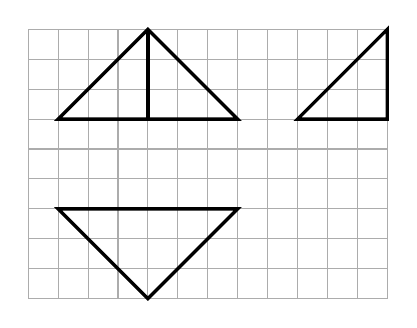
\begin{tikzpicture}[scale=.38]
  \draw[gray!65] (0,0) grid (12,9);
  \draw[very thick] (1,6)--(7,6)--(4,9)--cycle;
  \draw[very thick] (4,6)--(4,9);
  \draw[very thick] (9,6)--(12,6)--(12,9)--cycle;
  \draw[very thick] (1,3)--(7,3)--(4,0)--cycle;
\end{tikzpicture}
\end{center}
\nopagebreak[4]
\begin{gkopts}(4)
\task （A）$6$
\task （B）$9$
\task （C）$12$
\task （D）$18$
\end{gkopts}

\Needspace{4\baselineskip}
\textbf{解析}

\Needspace{5\baselineskip}
由三视图可识别出该几何体为底面为直角三角形、两直角边长为 $3,3$、高为 $6$ 的三棱锥。因此
\nopagebreak[4]
\[
V=\frac13\cdot\frac12\cdot3\cdot3\cdot6=9,
\]
选 B。

\gkanswer{答案：B}

\end{answer}
\begin{answer}
\gksolhead{8}{}

\textbf{题目}：

平面 $\alpha$ 截球 $O$ 的球面所得圆的半径为 $1$，球心 $O$ 到平面 $\alpha$ 的距离为 $\sqrt2$，则此球的体积为\mbox{（　　）}

\begin{gkopts}(4)
\task （A）$\sqrt6\pi$
\task （B）$4\sqrt3\pi$
\task （C）$4\sqrt6\pi$
\task （D）$6\sqrt3\pi$
\end{gkopts}

\Needspace{4\baselineskip}
\textbf{解析}

\Needspace{5\baselineskip}
设球半径为 $R$，球心到截面圆心的连线垂直于平面 $\alpha$，故
\nopagebreak[4]
\[
R^2=1^2+(\sqrt2)^2=3.
\]
\Needspace{5\baselineskip}
所以球体积为
\nopagebreak[4]
\[
V=\frac43\pi R^3=\frac43\pi(\sqrt3)^3=4\sqrt3\pi,
\]
选 B。

\gkanswer{答案：B}

\end{answer}
\begin{answer}
\gksolhead{9}{}

\textbf{题目}：

已知 $\omega>0$，$0<\varphi<\pi$，直线 $x=\dfrac\pi4$ 和 $x=\dfrac{5\pi}4$ 是函数 $f(x)=\sin(\omega x+\varphi)$ 图象的两条相邻的对称轴，则 $\varphi=$\mbox{（　　）}

\begin{gkopts}(2)
\task （A）$\dfrac\pi4$
\task （B）$\dfrac\pi3$
\task （C）$\dfrac\pi2$
\task （D）$\dfrac{3\pi}4$
\end{gkopts}

\Needspace{4\baselineskip}
\textbf{解析}

\Needspace{5\baselineskip}
正弦函数相邻对称轴的距离为 $\pi/\omega$，由
\nopagebreak[4]
\[
\frac{5\pi}4-\frac\pi4=\pi
\]
得 $\omega=1$。对称轴满足 $x+\varphi=\pi/2+k\pi$，结合 $0<\varphi<\pi$ 得 $\varphi=\pi/4$，选 A。

\gkanswer{答案：A}

\end{answer}
\begin{answer}
\gksolhead{10}{}

\textbf{题目}：

等轴双曲线 $C$ 的中心在原点，焦点在 $x$ 轴上，$C$ 与抛物线 $y^2=16x$ 的准线交于 $A,B$ 两点，$|AB|=4\sqrt3$，则 $C$ 的实轴长为\mbox{（　　）}

\begin{gkopts}(4)
\task （A）$\sqrt2$
\task （B）$2\sqrt2$
\task （C）$4$
\task （D）$8$
\end{gkopts}

\Needspace{4\baselineskip}
\textbf{解析}

\Needspace{5\baselineskip}
等轴双曲线可写为
\nopagebreak[4]
\[
\frac{x^2}{a^2}-\frac{y^2}{a^2}=1.
\]
\Needspace{5\baselineskip}
抛物线 $y^2=16x$ 的准线为 $x=-4$。代入双曲线，交点纵坐标满足
\nopagebreak[4]
\[
\frac{16-y^2}{a^2}=1.
\]
由 $|AB|=4\sqrt3$ 得 $y=\pm2\sqrt3$，从而 $16-12=a^2$，即 $a=2$。实轴长为 $2a=4$，选 C。

\gkanswer{答案：C}

\end{answer}
\begin{answer}
\gksolhead{11}{}

\textbf{题目}：

当 $0<x\leqslant\dfrac12$ 时，$4^x<\log_a x$，则 $a$ 的取值范围是\mbox{（　　）}

\begin{gkopts}(2)
\task （A）$\left(0,\dfrac{\sqrt2}{2}\right)$
\task （B）$\left(\dfrac{\sqrt2}{2},1\right)$
\task （C）$(1,\sqrt2)$
\task （D）$(\sqrt2,2)$
\end{gkopts}

\Needspace{4\baselineskip}
\textbf{解析}

\Needspace{5\baselineskip}
令 $c=-\ln a$。不等式要求 $a<1$，且
\nopagebreak[4]
\[
\frac{-\ln x}{c}>4^x\quad(0<x\leqslant1/2).
\]
\Needspace{5\baselineskip}
函数 $(-\ln x)/4^x$ 在该区间上递减，故最小值在 $x=1/2$ 处，得到
\nopagebreak[4]
\[
c<\frac{\ln2}{2},
\]
即 $\sqrt2/2<a<1$，选 B。

\gkanswer{答案：B}

\end{answer}
\begin{answer}
\gksolhead{12}{}

\textbf{题目}：

数列 $\{a_n\}$ 满足 $a_{n+1}+(-1)^n a_n=2n-1$，则 $\{a_n\}$ 的前 $60$ 项和为\mbox{（　　）}

\begin{gkopts}(4)
\task （A）$3690$
\task （B）$3660$
\task （C）$1845$
\task （D）$1830$
\end{gkopts}

\Needspace{4\baselineskip}
\textbf{解析}

\Needspace{5\baselineskip}
由递推式分别取奇、偶下标，得
\nopagebreak[4]
\[
a_{2k}-a_{2k-1}=4k-3,\qquad a_{2k+1}+a_{2k}=4k-1.
\]
\Needspace{5\baselineskip}
消去 $a_{2k}$ 后有 $a_{2k+1}=2-a_{2k-1}$，所以奇数项交替为 $a_1,2-a_1$。于是
\nopagebreak[4]
\[
\begin{aligned}
\sum_{n=1}^{60}a_n
&=\sum_{k=1}^{30}(a_{2k-1}+a_{2k})\\
&=\sum_{k=1}^{30}\bigl(2a_{2k-1}+4k-3\bigr)\\
&=15\cdot2a_1+15\cdot2(2-a_1)+\sum_{k=1}^{30}(4k-3)\\
&=60+1770=1830.
\end{aligned}
\]
选 D。

\gkanswer{答案：D}

\end{answer}
\begin{answer}
\gksolhead{13}{}

\textbf{题目}：

曲线 $y=x(3\ln x+1)$ 在点 $(1,1)$ 处的切线方程为\gkblank{}。

\Needspace{4\baselineskip}
\textbf{解析}

\nopagebreak[4]
\[
y'=3\ln x+4,
\]
故在 $(1,1)$ 处斜率为 $4$，切线方程为 $y-1=4(x-1)$，即 $y=4x-3$。

\gkanswer{答案：$y=4x-3$}

\end{answer}
\begin{answer}
\gksolhead{14}{}

\textbf{题目}：

等比数列 $\{a_n\}$ 的前 $n$ 项和为 $S_n$，若 $S_3+3S_2=0$，则公比 $q=$\gkblank{}。

\Needspace{4\baselineskip}
\textbf{解析}

\Needspace{5\baselineskip}
设首项为 $a_1$，公比为 $q$。由
\nopagebreak[4]
\[
S_3+3S_2=a_1(1+q+q^2)+3a_1(1+q)=a_1(q+2)^2=0,
\]
在等比数列首项非零的约定下，得 $q=-2$。

\gkanswer{答案：$-2$}

\end{answer}
\begin{answer}
\gksolhead{15}{}

\textbf{题目}：

已知向量 $\boldsymbol a,\boldsymbol b$ 夹角为 $45^\circ$，且 $|\boldsymbol a|=1$，$|2\boldsymbol a-\boldsymbol b|=\sqrt{10}$，则 $|\boldsymbol b|=$\gkblank{}。

\Needspace{4\baselineskip}
\textbf{解析}

\Needspace{5\baselineskip}
由夹角公式，令 $|\boldsymbol b|=t>0$，则
\nopagebreak[4]
\[
10=|2\boldsymbol a-\boldsymbol b|^2
=4+t^2-4t\cos45^\circ
=4+t^2-2\sqrt2t.
\]
所以 $t^2-2\sqrt2t-6=0$，取正根得 $|\boldsymbol b|=3\sqrt2$。

\gkanswer{答案：$3\sqrt2$}

\end{answer}
\begin{answer}
\gksolhead{16}{}

\textbf{题目}：

设函数 $f(x)=\dfrac{(x+1)^2+\sin x}{x^2+1}$ 的最大值为 $M$，最小值为 $m$，则 $M+m=$\gkblank{}。

\Needspace{4\baselineskip}
\textbf{解析}

\Needspace{5\baselineskip}
写成
\nopagebreak[4]
\[
f(x)=1+\frac{2x+\sin x}{x^2+1}.
\]
第二项是奇函数，故其最大值与最小值互为相反数，$M+m=2$。

\gkanswer{答案：$2$}

\end{answer}
\begin{answer}
\gksolhead{17}{}

\textbf{题目}：

已知 $a,b,c$ 分别为 $\triangle ABC$ 三个内角 $A,B,C$ 的对边，$a\cos C+\sqrt3a\sin C-b-c=0$。

（1）　求 $A$；

（2）　若 $a=2$，$\triangle ABC$ 的面积为 $\sqrt3$，求 $b,c$。

\Needspace{4\baselineskip}
\textbf{解析}

\gksubpart{(1) 证明}

\Needspace{5\baselineskip}
由正弦定理除以公共的 $2R$，原式化为
\nopagebreak[4]
\[
2\sin A\sin\left(C+\frac\pi6\right)=\sin B+\sin C.
\]
\Needspace{5\baselineskip}
利用 $A+B+C=\pi$，右端为 $\sin(A+C)+\sin C$。展开并约去正因子 $2\cos(A/2)$，得到
\nopagebreak[4]
\[
\sin C\left(\sqrt3\sin\frac A2-\cos\frac A2\right)=0.
\]
由于 $0<C<\pi$，所以 $\tan(A/2)=1/\sqrt3$，从而 $A=60^\circ$。

\gksubpart{(2) 解}

\Needspace{5\baselineskip}
面积条件给出
\nopagebreak[4]
\[
\frac12bc\sin60^\circ=\sqrt3,
\]
\Needspace{5\baselineskip}
即 $bc=4$。余弦定理给出
\nopagebreak[4]
\[
4=b^2+c^2-2bc\cos60^\circ=b^2+c^2-4,
\]
故 $b^2+c^2=8$。于是 $(b-c)^2=0$，所以 $b=c=2$。

\gkanswer{答案（1）：见解析版}

\gkanswer{答案（2）：$b=c=2$。}

\end{answer}
\begin{answer}
\gksolhead{18}{}

\textbf{题目}：

某花店每天以每枝 $5$ 元的价格从农场购进若干枝玫瑰花，然后以每枝 $10$ 元的价格出售，如果当天卖不完，剩下的玫瑰花作垃圾处理。

（1）　若花店一天购进 $16$ 枝玫瑰花，求当天的利润 $y$（单位：元）关于当天需求量 $n$（单位：枝，$n\in\mathbb N$）的函数解析式；

（2）　花店记录了 $100$ 天玫瑰花的日需求量（单位：枝），整理得下表：

\begin{center}
\begingroup\setlength{\tabcolsep}{4pt}
\begin{tabular}{lrrrrrrr}
\toprule
日需求量 $n$ & 14 & 15 & 16 & 17 & 18 & 19 & 20 \\
\midrule
频数 & 10 & 20 & 16 & 16 & 15 & 13 & 10 \\
\bottomrule
\end{tabular}
\endgroup
\end{center}

以 $100$ 天记录的各需求量的频率作为各需求量发生的概率。

① 假设花店在这 $100$ 天内每天购进 $17$ 枝玫瑰花，求这 $100$ 天的日利润（单位：元）的平均数；

② 若花店一天购进 $17$ 枝玫瑰花，以 $100$ 天记录的各需求量的频率作为各需求量发生的概率，求当天的利润不少于 $75$ 元的概率。

\Needspace{4\baselineskip}
\textbf{解析}

\gksubpart{(1) 解}

\Needspace{5\baselineskip}
购进 $16$ 枝的成本为 $80$ 元。当 $n\leqslant16$ 时售出 $n$ 枝，当 $n>16$ 时售出 $16$ 枝，因此
\nopagebreak[4]
\[
y=\begin{cases}10n-80,&n\leqslant16,\\80,&n>16.\end{cases}
\]

\gksubpart{(2) 解}

\Needspace{5\baselineskip}
每天购进 $17$ 枝时，需求量为 $14,15,16$ 的利润分别为 $55,65,75$ 元，需求量不小于 $17$ 时利润均为 $85$ 元。因此平均利润为
\nopagebreak[4]
\[
\frac{10\cdot55+20\cdot65+16\cdot75+(16+15+13+10)\cdot85}{100}=76.4.
\]
\Needspace{5\baselineskip}
利润不少于 $75$ 元对应需求量不小于 $16$，概率为
\nopagebreak[4]
\[
\frac{16+16+15+13+10}{100}=0.7.
\]

\gkanswer{答案（1）：$y=\begin{cases}10n-80,&n\leqslant16,\\80,&n>16;\end{cases}$}

\gkanswer{答案（2）：① $76.4$ 元；② $0.7$。}

\end{answer}
\begin{answer}
\gksolhead{19}{}

\textbf{题目}：

如图，三棱柱 $ABC-A_1B_1C_1$ 中，侧棱垂直底面，$\angle ACB=90^\circ$，$AC=BC=\dfrac12AA_1$，$D$ 是棱 $AA_1$ 的中点。

（1）　证明：平面 $BDC_1\perp$ 平面 $BDC$；

（2）　平面 $BDC_1$ 分此棱柱为两部分，求这两部分体积的比。

\Needspace{4\baselineskip}
\textbf{解析}

\gksubpart{(1) 证明}

\Needspace{5\baselineskip}
取 $a=AC=BC$，则 $AA_1=2a$。建立直角坐标系，令
\nopagebreak[4]
\[
C=(0,0,0),\quad A=(a,0,0),\quad B=(0,a,0),\quad C_1=(0,0,2a),
\]
\Needspace{5\baselineskip}
并有 $D=(a,0,a)$。平面 $BDC$、$BDC_1$ 的法向量可分别取
\nopagebreak[4]
\[
\boldsymbol n_1=\overrightarrow{BD}\times\overrightarrow{DC}=a^2(-1,0,1),
\qquad
\boldsymbol n_2=\overrightarrow{BD}\times\overrightarrow{DC_1}=a^2(1,2,1).
\]
\Needspace{5\baselineskip}
于是
\nopagebreak[4]
\[
\boldsymbol n_1\cdot\boldsymbol n_2=a^4(-1+1)=0,
\]
故两平面垂直。

\gksubpart{(2) 解}

\Needspace{5\baselineskip}
在上述坐标中，平面 $BDC_1$ 的方程为
\nopagebreak[4]
\[
x+2y+z=2a.
\]
\Needspace{5\baselineskip}
棱柱可表示为 $x\geqslant0,y\geqslant0,x+y\leqslant a,0\leqslant z\leqslant2a$。平面下方部分的高度为 $2a-x-2y$，其体积为
\nopagebreak[4]
\[
\int_0^a\int_0^{a-x}(2a-x-2y)\,dy\,dx=\frac12a^3.
\]
棱柱总体积为 $\frac12a^2\cdot2a=a^3$，故另一部分体积也为 $\frac12a^3$，两部分体积比为 $1:1$。

\gkanswer{答案（1）：见解析版}

\gkanswer{答案（2）：$1:1$。}

\end{answer}
\begin{answer}
\gksolhead{20}{}

\textbf{题目}：

设抛物线 $C:x^2=2py$（$p>0$）的焦点为 $F$，准线为 $l$，$A$ 为 $C$ 上一点，已知以 $F$ 为圆心、$FA$ 为半径的圆 $F$ 交 $l$ 于 $B,D$ 两点。

（1）　若 $\angle BFD=90^\circ$，$\triangle ABD$ 的面积为 $4\sqrt2$，求 $p$ 的值及圆 $F$ 的方程；

（2）　若 $A,B,F$ 三点在同一直线 $m$ 上，直线 $n$ 与 $m$ 平行，且 $n$ 与 $C$ 只有一个公共点，求坐标原点到 $m,n$ 距离的比值。

\Needspace{4\baselineskip}
\textbf{解析}

\gksubpart{(1) 解}

\Needspace{5\baselineskip}
焦点为 $F(0,p/2)$，准线为 $y=-p/2$。设圆半径为 $r=FA$。弦 $BD$ 所在直线到圆心的距离为 $p$，由 $\angle BFD=90^\circ$，有
\nopagebreak[4]
\[
2\sqrt{r^2-p^2}=r\sqrt2,
\]
\Needspace{5\baselineskip}
所以 $r=p\sqrt2$。抛物线的焦半径等于点到准线的距离，因而 $A$ 到准线的距离为 $p\sqrt2$。又 $BD=r\sqrt2=2p$，故
\nopagebreak[4]
\[
4\sqrt2=S_{\triangle ABD}=\frac12\cdot2p\cdot p\sqrt2=p^2\sqrt2,
\]
得到 $p=2$。此时 $F=(0,1)$、$r=2\sqrt2$，圆方程为 $x^2+(y-1)^2=8$。

\gksubpart{(2) 解}

\Needspace{5\baselineskip}
由 $A,B,F$ 共线，且 $A$ 在抛物线上、$B$ 在准线上，可得 $A=(\sqrt3p,3p/2)$（取另一侧只改变斜率符号）。于是
\nopagebreak[4]
\[
m:\ y=\frac{x}{\sqrt3}+\frac p2.
\]
\Needspace{5\baselineskip}
原点到 $m$ 的距离为 $\sqrt3p/4$。与其平行且与抛物线相切的直线为
\nopagebreak[4]
\[
n:\ y=\frac{x}{\sqrt3}-\frac p6,
\]
原点到 $n$ 的距离为 $\sqrt3p/12$。所求比值为 $3:1$。

\gkanswer{答案（1）：$p=2$，圆 $F$ 的方程为 $x^2+(y-1)^2=8$。}

\gkanswer{答案（2）：$3:1$。}

\end{answer}
\begin{answer}
\gksolhead{21}{}

\textbf{题目}：

设函数 $f(x)=\mathrm e^x-ax-2$。

（1）　求 $f(x)$ 的单调区间；

（2）　若 $a=1$，$k$ 为整数，且当 $x>0$ 时，$(x-k)f'(x)+x+1>0$，求 $k$ 的最大值。

\Needspace{4\baselineskip}
\textbf{解析}

\gksubpart{(1) 解}

\nopagebreak[4]
\[
f'(x)=\mathrm e^x-a.
\]
当 $a\leqslant0$ 时，$f'(x)>0$，函数在 $\mathbb R$ 上单调递增；当 $a>0$ 时，$f'(x)$ 在 $x=\ln a$ 处变号，函数在 $(-\infty,\ln a)$ 上单调递减，在 $(\ln a,+\infty)$ 上单调递增。

\gksubpart{(2) 解}

\Needspace{5\baselineskip}
取 $a=1$，不等式化为
\nopagebreak[4]
\[
(x-k)(\mathrm e^x-1)+x+1=(x-k)\mathrm e^x+k+1>0.
\]
当 $k\leqslant1$ 时该式从 $x=0$ 附近的值 $1$ 开始递增；对 $k=2$，其极小值在 $x=1$，为 $3-\mathrm e>0$。而 $k=3$ 时在 $x=2$ 处取值 $4-\mathrm e^2<0$。故 $k$ 的最大值为 $2$。

\gkanswer{答案（1）：当 $a\leqslant0$ 时在 $\mathbb R$ 上单调递增；当 $a>0$ 时在 $(-\infty,\ln a)$ 上单调递减，在 $(\ln a,+\infty)$ 上单调递增。}

\gkanswer{答案（2）：$k$ 的最大值为 $2$。}

\end{answer}
\begin{answer}
\gksolhead{22}{}

\textbf{题目}：

如图，$D,E$ 分别为 $\triangle ABC$ 边 $AB,AC$ 的中点，直线 $DE$ 交 $\triangle ABC$ 的外接圆于 $F,G$ 两点。若 $CF\parallel AB$，证明：

（1）　$CD=BC$；

（2）　$\triangle BCD\sim\triangle GBD$。
\nopagebreak[4]
\begin{center}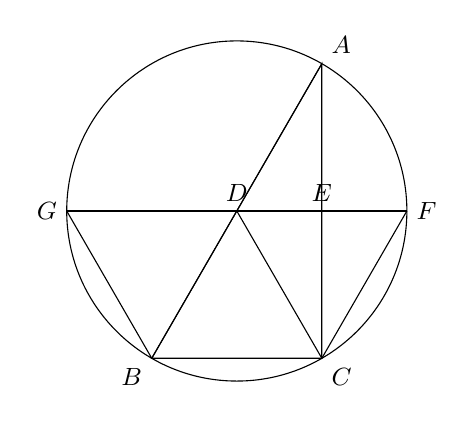
\begin{tikzpicture}[scale=.72, every node/.style={font=\small}]
  \coordinate (G) at (-3,0);
  \coordinate (F) at (3,0);
  \coordinate (A) at (1.5,2.598);
  \coordinate (B) at (-1.5,-2.598);
  \coordinate (C) at (1.5,-2.598);
  \coordinate (D) at (0,0);
  \coordinate (E) at (1.5,0);
  \draw (0,0) circle (3);
  \draw (G)--(F);
  \draw (A)--(B)--(C)--cycle;
  \draw (D)--(C);
  \draw (G)--(B);
  \draw (C)--(F);
  \draw (A)--(C);
  \draw (A)--(B);
  \node[above right] at (A) {$A$};
  \node[below left] at (B) {$B$};
  \node[below right] at (C) {$C$};
  \node[above] at (D) {$D$};
  \node[above] at (E) {$E$};
  \node[left] at (G) {$G$};
  \node[right] at (F) {$F$};
\end{tikzpicture}
\end{center}
\nopagebreak[4]
\Needspace{4\baselineskip}
\textbf{解析}

\gksubpart{(1) 证明}

\Needspace{5\baselineskip}
设 $B=(0,0)$、$C=(1,0)$、$A=(u,v)$，其中 $v>0$。则
\nopagebreak[4]
\[
D=\left(\frac u2,\frac v2\right),\qquad E=\left(\frac{u+1}2,\frac v2\right).
\]
\Needspace{5\baselineskip}
圆 $ABC$ 的方程可写为 $x^2+y^2-x+\lambda y=0$。直线 $CF\parallel AB$ 与 $y=v/2$ 的交点参数为 $1/2$，代入圆方程得到
\nopagebreak[4]
\[
u^2+v^2=4u.
\]
\Needspace{5\baselineskip}
于是
\nopagebreak[4]
\[
CD^2=\left(\frac u2-1\right)^2+\frac{v^2}{4}=1=BC^2,
\]
故 $CD=BC$。

\gksubpart{(2) 证明}

\Needspace{5\baselineskip}
直线 $DE$ 与圆的两个交点横坐标之和为 $1$，而由上式其中一个交点为 $F=(1+u/2,v/2)$，故另一个为 $G=(-u/2,v/2)$。因此
\nopagebreak[4]
\[
GD=u,\qquad GB=BD=\frac12\sqrt{u^2+v^2}=\sqrt u,\qquad BC=CD=1.
\]
\Needspace{5\baselineskip}
从而
\nopagebreak[4]
\[
\frac{BC}{BD}=\frac{CD}{GB}=\frac{BD}{GD}=\frac1{\sqrt u},
\]
故 $\triangle BCD\sim\triangle GBD$。

\gkanswer{答案（1）：见解析版}

\gkanswer{答案（2）：见解析版}

\end{answer}
\begin{answer}
\gksolhead{23}{}

\textbf{题目}：

已知曲线 $C_1$ 的参数方程是 $\begin{cases}x=2\cos\varphi,\\y=3\sin\varphi,\end{cases}$（$\varphi$ 是参数）．以坐标原点为极点，$x$ 轴的非负半轴为极轴建立极坐标系，曲线 $C_2$ 的极坐标方程是 $\rho=2$，正方形 $ABCD$ 的顶点都在 $C_2$ 上，且 $A,B,C,D$ 依逆时针次序排列，点 $A$ 的极坐标为 $(2,\dfrac\pi3)$。

（1）　求点 $A,B,C,D$ 的直角坐标；

（2）　设 $P$ 为 $C_1$ 上任意一点，求 $|PA|^2+|PB|^2+|PC|^2+|PD|^2$ 的取值范围。

\Needspace{4\baselineskip}
\textbf{解析}

\gksubpart{(1) 解}

\Needspace{5\baselineskip}
正方形外接圆半径为 $2$，相邻顶点的极角相差 $\pi/2$。依逆时针顺序，四点极角为
\nopagebreak[4]
\[
\frac\pi3,\quad\frac{5\pi}6,\quad\frac{4\pi}3,\quad\frac{11\pi}6.
\]
\Needspace{5\baselineskip}
所以
\nopagebreak[4]
\[
A=(1,\sqrt3),\quad B=(-\sqrt3,1),\quad C=(-1,-\sqrt3),\quad D=(\sqrt3,-1).
\]

\gksubpart{(2) 解}

\Needspace{5\baselineskip}
设 $P=(x,y)$。正方形四个顶点的坐标和为零，且每个顶点到原点的距离平方为 $4$，故
\nopagebreak[4]
\[
\begin{aligned}
&|PA|^2+|PB|^2+|PC|^2+|PD|^2\\
&=4(x^2+y^2)+16.
\end{aligned}
\]
\Needspace{5\baselineskip}
由参数方程 $x=2\cos\varphi,y=3\sin\varphi$，有
\nopagebreak[4]
\[
4(x^2+y^2)+16=16\cos^2\varphi+36\sin^2\varphi+16.
\]
故取值范围为 $[32,52]$。

\gkanswer{答案（1）：$A(1,\sqrt3)$，$B(-\sqrt3,1)$，$C(-1,-\sqrt3)$，$D(\sqrt3,-1)$。}

\gkanswer{答案（2）：$[32,52]$。}

\end{answer}
\begin{answer}
\gksolhead{24}{}

\textbf{题目}：

已知函数 $f(x)=|x+a|+|x-2|$。

（1）　当 $a=-3$ 时，求不等式 $f(x)\geqslant3$ 的解集；

（2）　若 $f(x)\leqslant|x-4|$ 的解集包含 $[1,2]$，求 $a$ 的取值范围。

\Needspace{4\baselineskip}
\textbf{解析}

\gksubpart{(1) 解}

\Needspace{5\baselineskip}
当 $a=-3$ 时，$f(x)=|x-3|+|x-2|$。分 $x\leqslant2$、$2\leqslant x\leqslant3$、$x\geqslant3$ 讨论，分别得到
\nopagebreak[4]
\[
5-2x\geqslant3,\qquad1\geqslant3,\qquad2x-5\geqslant3.
\]
因此解集为 $(-\infty,1]\cup[4,+\infty)$。

\gksubpart{(2) 解}

\Needspace{5\baselineskip}
对 $x\in[1,2]$，原不等式等价于
\nopagebreak[4]
\[
|x+a|\leqslant2.
\]
\Needspace{5\baselineskip}
要使区间 $[1+a,2+a]$ 包含于 $[-2,2]$，必须且只需
\nopagebreak[4]
\[
1+a\geqslant-2,\qquad2+a\leqslant2.
\]
所以 $-3\leqslant a\leqslant0$。

\gkanswer{答案（1）：$(-\infty,1]\cup[4,+\infty)$。}

\gkanswer{答案（2）：$-3\leqslant a\leqslant0$。}

\end{answer}